\subsection{Задание 5. Сетевые возможности убунту.}


Сетвые возможности Ubuntu: подключение к локальной сети \ref{fig:conectToLocal}, к Wi"=Fi \ref{fig:conectToWiFi} %, использование сетевых протоколов \ref{fig:delDir} :

\begin{figure}[!h]
    \centering
    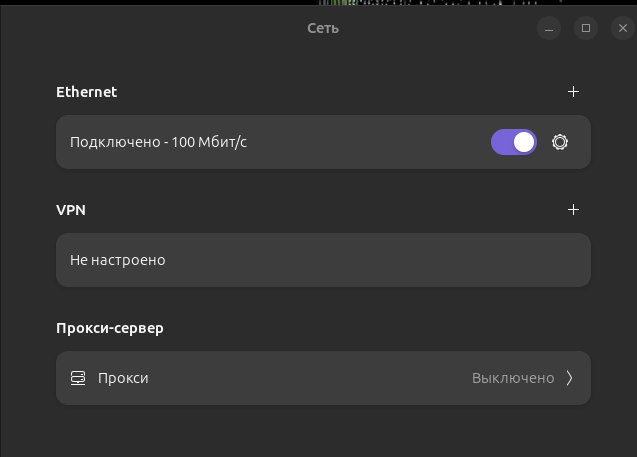
\includegraphics[width = 0.8\textwidth]{images/conectToLocal.png}
    
    \caption{Подключение к локальной сети}
    
    \label{fig:conectToLocal}
\end{figure}

\begin{figure}[!h]
    \centering
    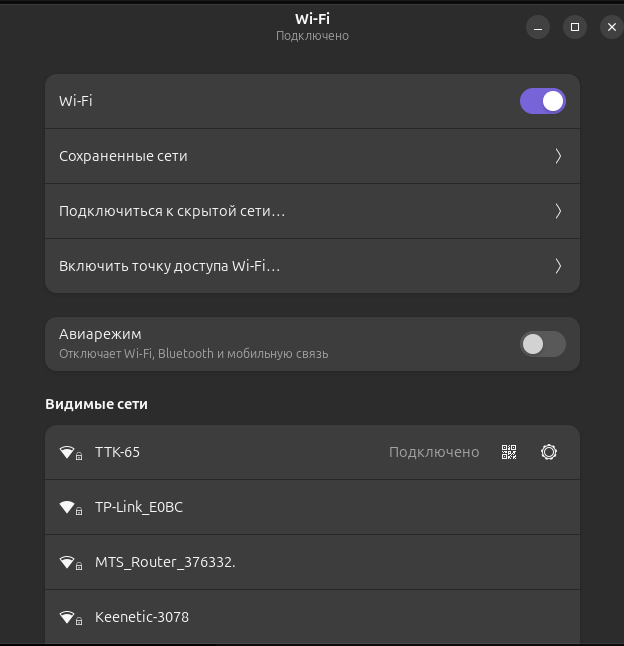
\includegraphics[width = 0.8\textwidth]{images/conectToWiFi.png}
    
    \caption{Подключение к Wi"=Fi}
    
    \label{fig:conectToWiFi}
\end{figure}

ifconfig \ref{fig:ifconfig}, ip \ref{fig:ipconf}

\begin{figure}[!h]
    \centering
    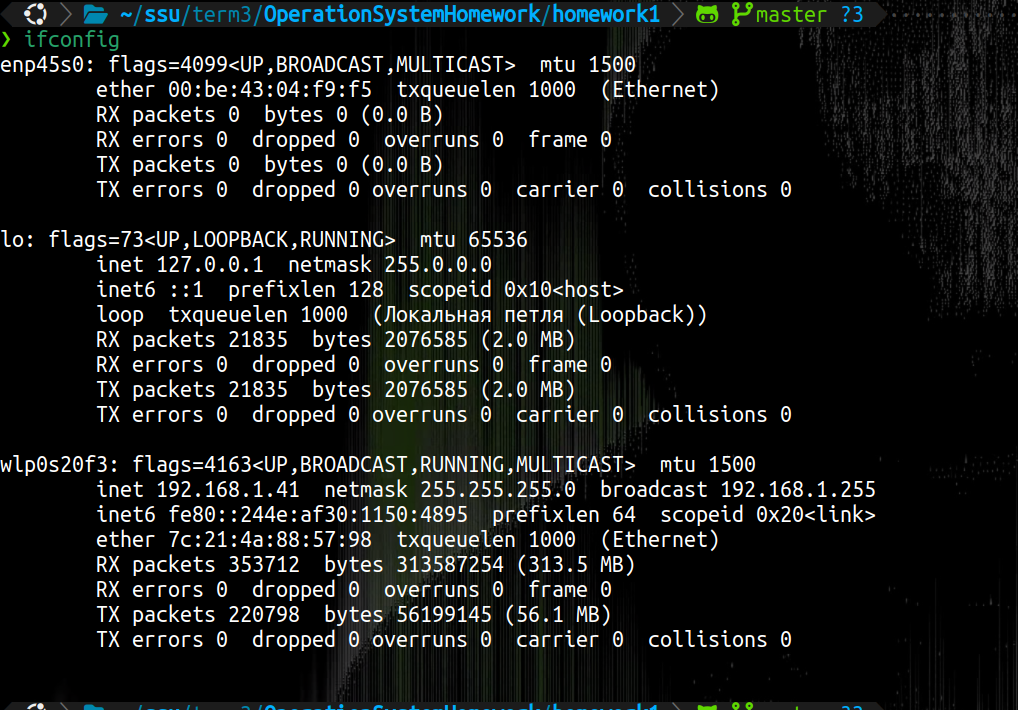
\includegraphics[width = 0.8\textwidth]{images/ifconfig.png}
    
    \caption{ifconfig}
    
    \label{fig:ifconfig}
\end{figure}

\begin{figure}[!h]
    \centering
    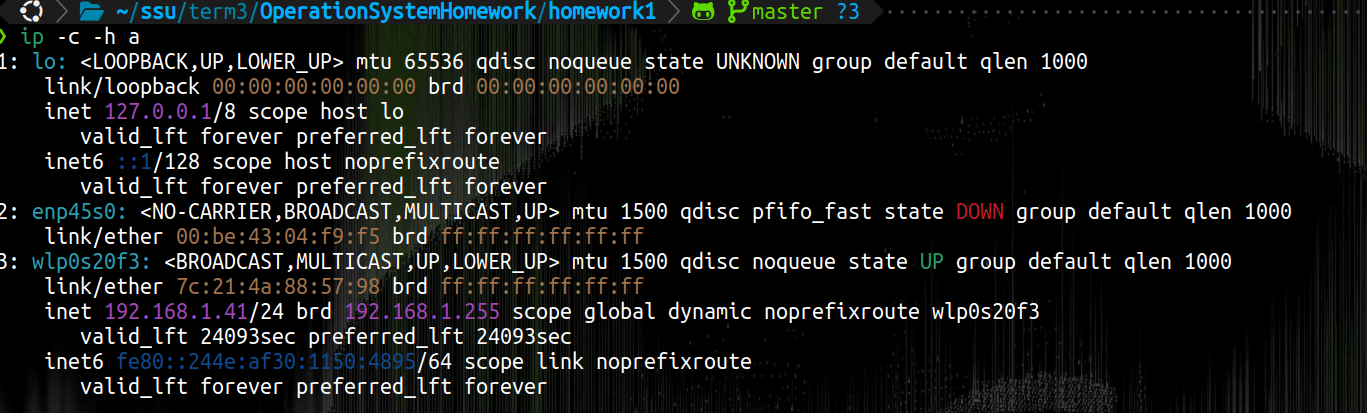
\includegraphics[width = 0.8\textwidth]{images/ipconf.png}
    
    \caption{ip}
    
    \label{fig:ipconf}
\end{figure}

ping \ref{fig:pingSGU}

\begin{figure}[!h]
    \centering
    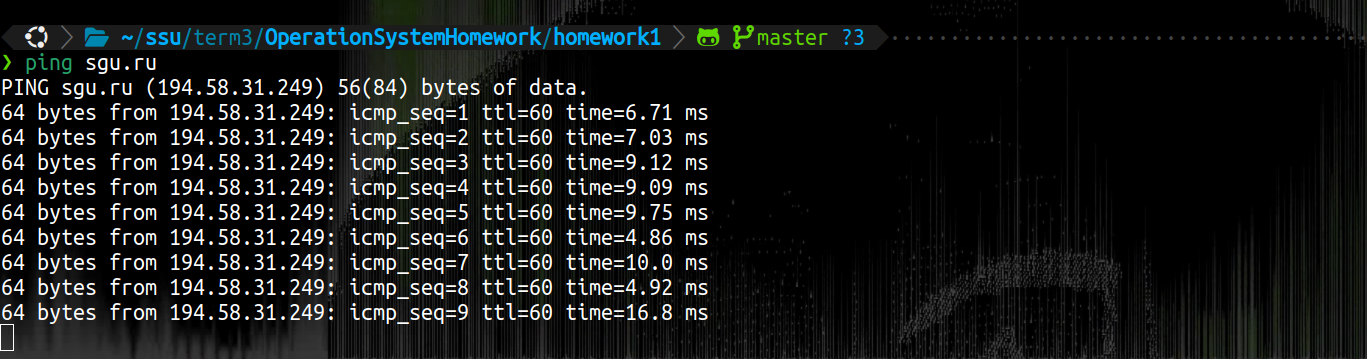
\includegraphics[width = 0.8\textwidth]{images/pingSGU.png}
    
    \caption{ping SGU}
    
    \label{fig:pingSGU}
\end{figure}

\newpage

